\documentclass{standalone}
\usepackage[T1]{fontenc}
\usepackage[utf8]{inputenc}
\usepackage{pgf,tikz}
\usepackage{setspace}
\usepackage{pgfplots}
\pgfplotsset{compat=1.13}

\begin{document}

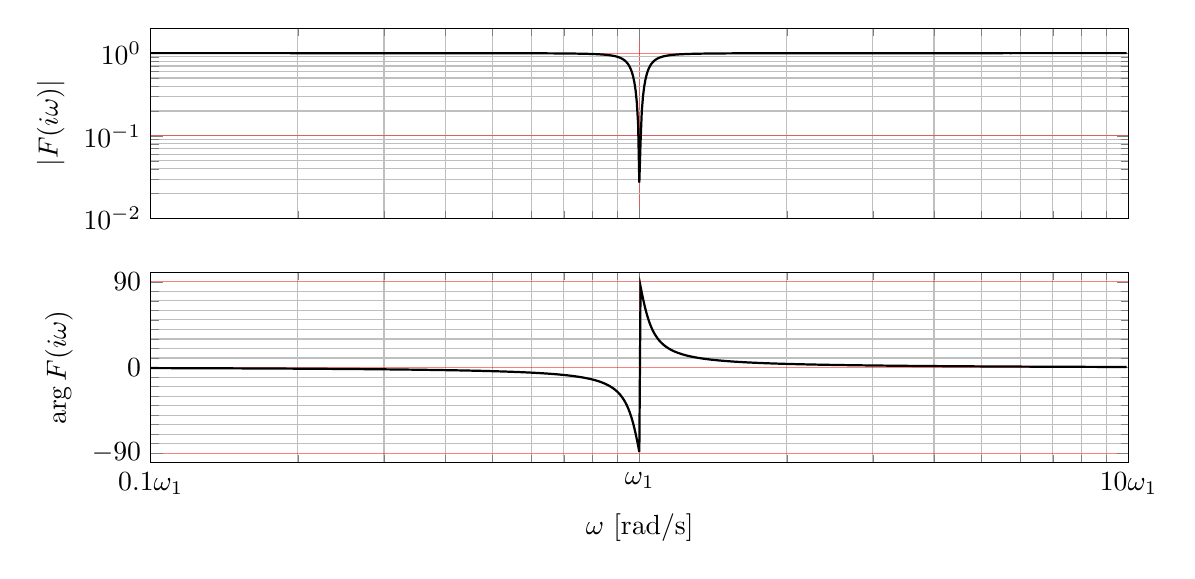
\begin{tikzpicture}
  \pgfmathsetmacro{\ww}{1}
  \pgfmathsetmacro{\QQ}{10}
  \pgfmathsetmacro{\zz}{1/2/\QQ}
  \pgfmathsetmacro{\zzcomp}{sqrt(1 - \zz*\zz)}
  \pgfmathsetmacro{\poleRe}{\zz*\ww}
  \pgfmathsetmacro{\poleIm}{\zzcomp*\ww}
  \pgfmathsetmacro{\poleReSq}{pow(\poleRe, 2)}

  \begin{semilogxaxis} [
      xlabel={$\omega$ [rad/s]},
      ylabel=$\arg F(i\omega)$,
      width=14cm,
      height=4cm,
      grid=both,
      every major grid/.style={red, opacity=0.5},
      ytick={-90, 0, 90},
      %yticklabels={$-45^\circ$, $0^\circ$, $45^\circ$}, 
      xtick={0.1, 1, 10},
      xticklabels={$0.1\omega_1$, $\omega_1$, $10\omega_1$},
      ymin=-100, ymax=100,
      xmin=0.1, xmax=10,
      minor y tick num=8,
      %legend entries={Bessel filter, Delay of one},
      %legend pos={south west},
  ]
  \addplot[thick, black, no marks, domain=0.1:10, samples=800] { (x>\ww)*180 - atan2(x+\poleIm, \poleRe) - atan2(x-\poleIm, \poleRe) };
  \end{semilogxaxis}
  \begin{loglogaxis} [
      ylabel=$|F(i\omega)|$,
      yshift = 3.1cm, 
      width=14cm,
      height=4cm,
      grid=both,
      every major grid/.style={red, opacity=0.5},
      ytick={0.01, 0.1, 1},
      %yticklabels={$0.01\omega_1$, $0.1\omega_1$, $\omega_1$, $10\omega_1$},
      xticklabel=\empty,
      ymin=0.01, ymax=2,
      xmin=0.1, xmax=10,
      %legend entries={Bessel filter, Delay of one},
      %legend pos={south west},
  ]
 \addplot[thick, black, no marks, domain=0.1:10, samples=800] { abs(x+\ww)*abs(x-\ww)/sqrt(\poleReSq + pow(x+\poleIm, 2))/sqrt(\poleReSq + pow(x-\poleIm, 2))};
  \end{loglogaxis}

\end{tikzpicture}

\end{document}
